\documentclass[]{elsarticle} %review=doublespace preprint=single 5p=2 column
%%% Begin My package additions %%%%%%%%%%%%%%%%%%%
\usepackage[hyphens]{url}

  \journal{Astronomy \& Astrophysics} % Sets Journal name


\usepackage{lineno} % add
\providecommand{\tightlist}{%
  \setlength{\itemsep}{0pt}\setlength{\parskip}{0pt}}

\bibliographystyle{elsarticle-harv}
\biboptions{sort&compress} % For natbib
\usepackage{graphicx}
\usepackage{booktabs} % book-quality tables
%%%%%%%%%%%%%%%% end my additions to header

\usepackage[T1]{fontenc}
\usepackage{lmodern}
\usepackage{amssymb,amsmath}
\usepackage{ifxetex,ifluatex}
\usepackage{fixltx2e} % provides \textsubscript
% use upquote if available, for straight quotes in verbatim environments
\IfFileExists{upquote.sty}{\usepackage{upquote}}{}
\ifnum 0\ifxetex 1\fi\ifluatex 1\fi=0 % if pdftex
  \usepackage[utf8]{inputenc}
\else % if luatex or xelatex
  \usepackage{fontspec}
  \ifxetex
    \usepackage{xltxtra,xunicode}
  \fi
  \defaultfontfeatures{Mapping=tex-text,Scale=MatchLowercase}
  \newcommand{\euro}{€}
\fi
% use microtype if available
\IfFileExists{microtype.sty}{\usepackage{microtype}}{}
\usepackage{longtable}
\usepackage{graphicx}
% We will generate all images so they have a width \maxwidth. This means
% that they will get their normal width if they fit onto the page, but
% are scaled down if they would overflow the margins.
\makeatletter
\def\maxwidth{\ifdim\Gin@nat@width>\linewidth\linewidth
\else\Gin@nat@width\fi}
\makeatother
\let\Oldincludegraphics\includegraphics
\renewcommand{\includegraphics}[1]{\Oldincludegraphics[width=\maxwidth]{#1}}
\ifxetex
  \usepackage[setpagesize=false, % page size defined by xetex
              unicode=false, % unicode breaks when used with xetex
              xetex]{hyperref}
\else
  \usepackage[unicode=true]{hyperref}
\fi
\hypersetup{breaklinks=true,
            bookmarks=true,
            pdfauthor={},
            pdftitle={The Locus Algorithm},
            colorlinks=false,
            urlcolor=blue,
            linkcolor=magenta,
            pdfborder={0 0 0}}
\urlstyle{same}  % don't use monospace font for urls

\usepackage{xcolor}
\usepackage{graphicx}


%\setcounter{secnumdepth}{0}
%% Pandoc toggle for numbering sections (defaults to be off)
%\setcounter{secnumdepth}{0}
%% Pandoc header

\usepackage{caption}
\DeclareCaptionType{equ}[Expression][]

\begin{document}
\begin{frontmatter}

\title{The Locus Algorithm}


\author[DIAS,TUD]{Ois\'in Creaner\corref{cor1}}
\cortext[cor1]{Corresponding author}
\ead{creanero@cp.dias.ie}

\author[TUD]{Eugene Hickey}
\ead{Eugene.Hickey@it-tallaght.ie}
\author[TUD]{Kevin Nolan}
\ead{Kevin.Nolan@it-tallaght.ie}
\author[CIT]{Niall Smith}
\ead{nsmith@cit.ie}

\address[DIAS]{Dublin Institute for Advanced Studies, 31 Fitzwilliam Place, Dublin 2, Ireland}
\address[TUD]{Technological University Dublin, Tallaght Campus, Dublin 24, Ireland}
\address[CIT]{Cork Institute of Technology, Bishopstown, Cork, Ireland}

  
  \begin{abstract}
  This Paper describes the design, implementation and operation of a new algorithm,
  The Locus Algorithm; which enables optimised differential photometry.
  For a given target, The Locus Algorithm identifies the pointing for
  which the resultant FoV includes the target and the maximum number of
  similar reference stars available, thus enabling optimised differential
  photometry of the target. The application of The Locus
  Algorithm to a target from the Sloan Digital Sky Survey to provide
  optimum differential photometry for that target is also described. The algorithm was also
  used to generate catalogues of pointing's to optimise Quasars
  variability studies and to generate catalogues of optimised pointings in
  the search for Exoplanets via the transit method.
  \end{abstract}
  
 \end{frontmatter}

\hypertarget{introduction}{%
\section{Introduction}\label{introduction}}

Photometric variability studies involve identifying variations in
brightness of a celestial point source over time. Such studies are
hampered by the Earth's atmosphere, which causes first order and second
order extinction \citep{milone2011high,young1991precise}. Differential
Photometry mitigates the effect of the Earth's atmosphere by comparing
the brightness of a target to reference stars in the same Field of View
(FoV). Differential photometry can be optimised for the target by
choosing a pointing whose Field of View (FoV) includes the target and
the maximum number of reference stars of similar magnitude and colour.
\citep{milone2011high,young1991precise,howell2006handbook,honeycutt1992ccd}).

The Locus Algorithm enables optimised differential photometry by
identifying the pointing for which the resultant FoV includes the target
and the best set of similar reference stars available.

\hypertarget{conceptual-basis-to-the-locus-algorithm}{%
\section{Conceptual basis to The Locus
Algorithm}\label{conceptual-basis-to-the-locus-algorithm}}

A locus can be defined around any star such that a FoV centred on any
point on the locus will include the star at the edge of the FoV. For
fields containing stars close to one another, if one locus intersects
with another, they produce Points of Intersection (PoIs) as shown in Figure \ref{loci_concept}.

\begin{figure}
\centering
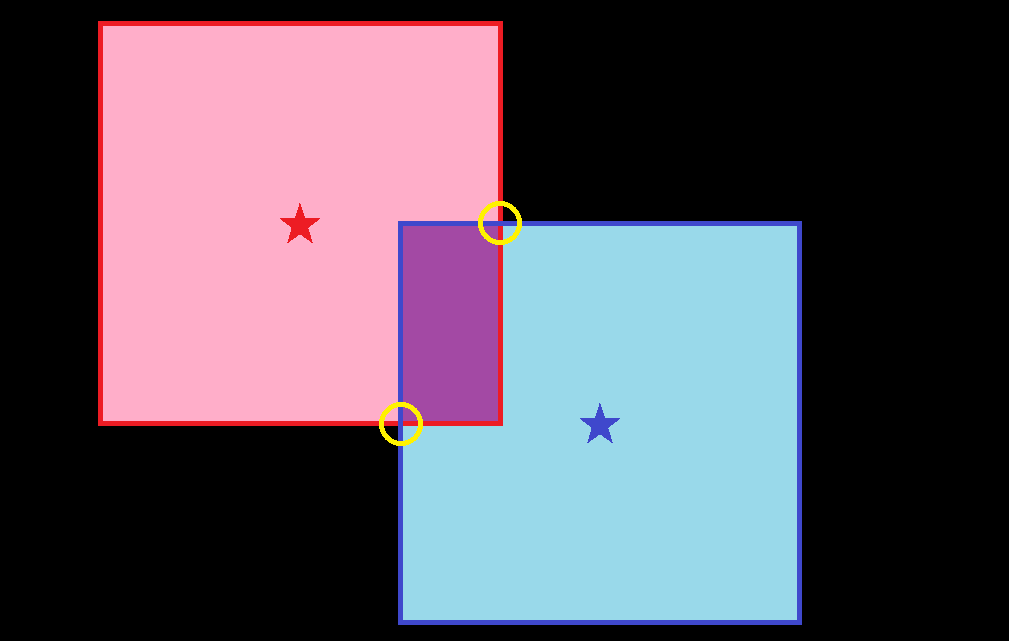
\includegraphics{fig1.png}
\caption{\label{loci_concept}Diagrammatic representation of two stars with loci
(red and blue perimeter lines), which intersect and produce two Points
of Intersection (PoI's) circled in yellow.  Copied from \citet{creaner2016thesis}}
\end{figure}

A FoV centred on any such PoI will include both stars associated with
creating it. At Points of Intersection the set of stars that can be
included in a FoV changes.

The Locus Algorithm considers candidate reference stars in what is
termed a Candidate Zone (CZ) - the zone of sky centred on the target
within which a FoV can be selected which includes both the reference
star and the target. For Candidate Reference Stars within the CZ, 
loci are determined, and all relevant PoI are identified. Each PoI 
is assigned a score derived from the number and similarity of reference
stars included in a FoV centred on that PoI. The PoI with the highest score 
becomes the pointing for the target.

\hypertarget{locus-algorithm-design}{%
\section{Locus Algorithm Design}\label{locus-algorithm-design}}
Based on the conceptual outline above, this section provides a mathematical
definition of the Locus Algorithm and an explanation of the terms used in it.
Section \ref{example-implementation-of-the-locus-algorithm} below describes a
 worked example of this algorithm applied to a sample star, SDSS ID 1237680117417115655.
\hypertarget{definition-of-coordinate-system-and-locus}{%
\subsection{Definition of Coordinate System and
Locus}\label{definition-of-coordinate-system-and-locus}}

For computational efficiency, The Locus Algorithm considers a Field of
View to be a rectangular area on the sky orientated such that the edges
are aligned with the primary x and y axes of the Cartesian coordinate
system. Movement of the field is restricted to x or y translations.

However, the Celestial coordinate system is defined by the Equatorial
coordinate system, with coordinates specified by Right Ascension (RA)
and Declination (Dec). Because this is a spherical coordinate system,
unit angle in RA is foreshortened, with the degree of foreshortening
defined in Expression \ref{RAshort}
\begin{equ}[!h]
  \begin{equation}
angle \in RA = {\frac{True Angle}{cos(Dec)}}
  \end{equation}
\caption{\label{RAshort}Right Ascension foreshortening with Declination}
\end{equ}

By using this conversion, it is possible to approximate to a high degree
of accuracy a Cartesian coordinate system using RA and Dec; with a small
FoV of East-West size \(R\) and North-South size \(S\) about a target located at
point \(RA_t\) and \(Dec_t\).  Expression \ref{Rprime} defines a corrected angular size in RA direction ($R^\prime$)

\begin{equ}[!h]
  \begin{equation}
R^\prime = {\frac{R}{cos(Dec_t)}}
  \end{equation}
\caption{\label{Rprime}Definition of a corrected angular size along the RA direction (R$^\prime$)}
\end{equ}

Given these terms, Expression \ref{FoVDef} defines the FoV.

\begin{equ}[!h]
\begin{equation}
\begin{split}
&RA_t - {\frac{R^\prime}{2}} \leq RA \leq RA_t + {\frac{R^\prime}{2}} \\
&Dec_t - {\frac{S}{2}} \leq Dec \leq Dec_t + {\frac{S}{2}}
\end{split}
\end{equation}
\caption{\label{FoVDef}Definition of a FoV of size R x S centred on a target at
(\(RA_t\) , \(Dec_t\))}
\end{equ}

This definition is accurate to approximately 1\% for a FoV of area 15$^\prime$
square outside celestial polar regions as shown in Expression \ref{polar}.

\begin{equ}[!h]
  \begin{equation}
\begin{split}
&Given: R, S = 15^\prime , \lvert Dec\rvert \leq 66.5 \textdegree\\
&{\frac{\lvert\frac{R}{cos(Dec-S)}-\frac{R}{cos(Dec+S)}\rvert}{\frac{R}{cos(Dec)}}}\leq 0.01
\end{split}
  \end{equation}
\caption{\label{polar}Evaluation of the accuracy of the R$^\prime$ for areas away from the celestial pole.}
\end{equ}

As expresed here, the formula does not consider RA ``loop
around'' from 359.99\textdegree  to 0.00\textdegree ; resulting, for
example, in the exclusion of 0.23\% of the SDSS catalogue. Planned
enhancements to The Locus Algorithm will resolve these shortcomings.

We can therefore define the locus about any star on the sky located at
\(RA_t\) and \(Dec_t\) as the values of Right Ascension and Declination
as defined in Equation 2.

\hypertarget{candidate-zone}{%
\subsection{Candidate Zone}\label{candidate-zone}}

A Candidate Zone is defined as a region centred on the target, equal to
four times the area of the Field of View, within which any
reference star can be included in a Field of View with the target and
can therefore be considered as a candidate reference star in identifying
the optimum pointing. Conversely, stars outside the candidate zone
cannot be included in a Field of View with the target and cannot
therefore be considered as candidates reference stars. Hence the
Candidate Zone is the maximum region of sky centred on the target from
which to choose candidate reference stars when identifying an optimum
pointing for a given target. For a target positioned at coordinates
\(RA_c\) and \(Dec_c\) the resulting Candidate Zone is defined by Expression \ref{CZdef}.
\begin{equ}[!h]
  \begin{equation}
\begin{split}
&RA_t - R^\prime \leq RA_r \leq RA_t + R^\prime \\
&Dec_t - S \leq Dec_r \leq Dec_t + S
\end{split}
  \end{equation}
\caption{\label{CZdef}Definition of a Candidate Zone of size 2R x 2S centred on a
target with coordinates (\(RA_t\), \(Dec_t\)), in which zone reference stars with coordinates (\(RA_r\), \(Dec_r\)) can be found.}
\end{equ}


%\begin{figure}
%\centering
%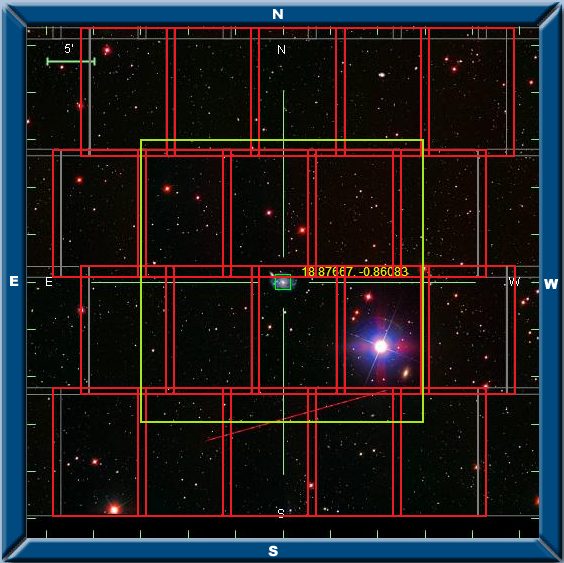
\includegraphics{fig2.png}
%\caption{Modified image taken from the SDSS ``Navigate'' tool.
%The image showing fields (in red) needed to form a mosaic from which a
%Candidate Zone (green) centred on the target can be defined.}
%\end{figure}

\hypertarget{identification-and-filtering-of-reference-stars}{%
\subsection{Identification and Filtering of Reference
Stars}\label{identification-and-filtering-of-reference-stars}}

For each target, a list of candidate reference stars in its Candidate
Zone is produced based on the following criteria:

\begin{itemize}
\tightlist
\item
  Position: the reference star must be in the Candidate Zone as defined in Expression \ref{CZdef}.
\item
  Magnitude: the magnitude of the reference star (\(mag_r\)) must be within a user-defined limit (\(\Delta mag\)) of the target's magnitude (\(mag_t\)) as shown in Expression \ref{maglim}.
\item
  Colour: the colour index (e.g. \(g-r\)) of the reference star (\(col_r\)) must match the colour of the target (\(col_t\)) to
  within a user-specified limit(\(\Delta col\)) as shown in Expression \ref{collim}.
\item
  Resolvability: the reference star must be resolvable, i.e.~no other
  star that would impact a brightness measurements within a
  user-specified resolution limit.
\end{itemize}

All stars in the Candidate Zone which pass these initial filters become
the list of candidate reference stars for which loci will be
identified.

\begin{equ}[!h]
  \begin{equation}
\begin{split}
&mag_t - \Delta mag \leq mag_c \leq mag_t + \Delta mag \\
\end{split}
  \end{equation}
\caption{\label{maglim}Definition of the limits of mag difference between the target and references.}
\end{equ}

\begin{equ}[!h]
  \begin{equation}
\begin{split}
&col_t - \Delta col \leq col_c \leq col_t + \Delta col \\
\end{split}
  \end{equation}
\caption{\label{collim}Definition of the limits of colour difference between the target and references.}
\end{equ}

\hypertarget{identifying-the-effective-locus-for-each-candidate-reference-star}{%
\subsection{Identifying the Effective Locus for each Candidate Reference
Star}\label{identifying-the-effective-locus-for-each-candidate-reference-star}}

The locus associated with each candidate reference star must be
identified based on Equation \ref{FoVDef}. For the purposes of identifying Points
of Intersection, only the side surrounding a given candidate reference
star closest to the target need be considered. Hence, we can define the
effective locus for such a candidate reference star as a single line of
constant RA and a single line of constant Dec nearest the target star
as shown in Figure \ref{effective_locus}.

\begin{figure}
\centering
\colorbox{black}{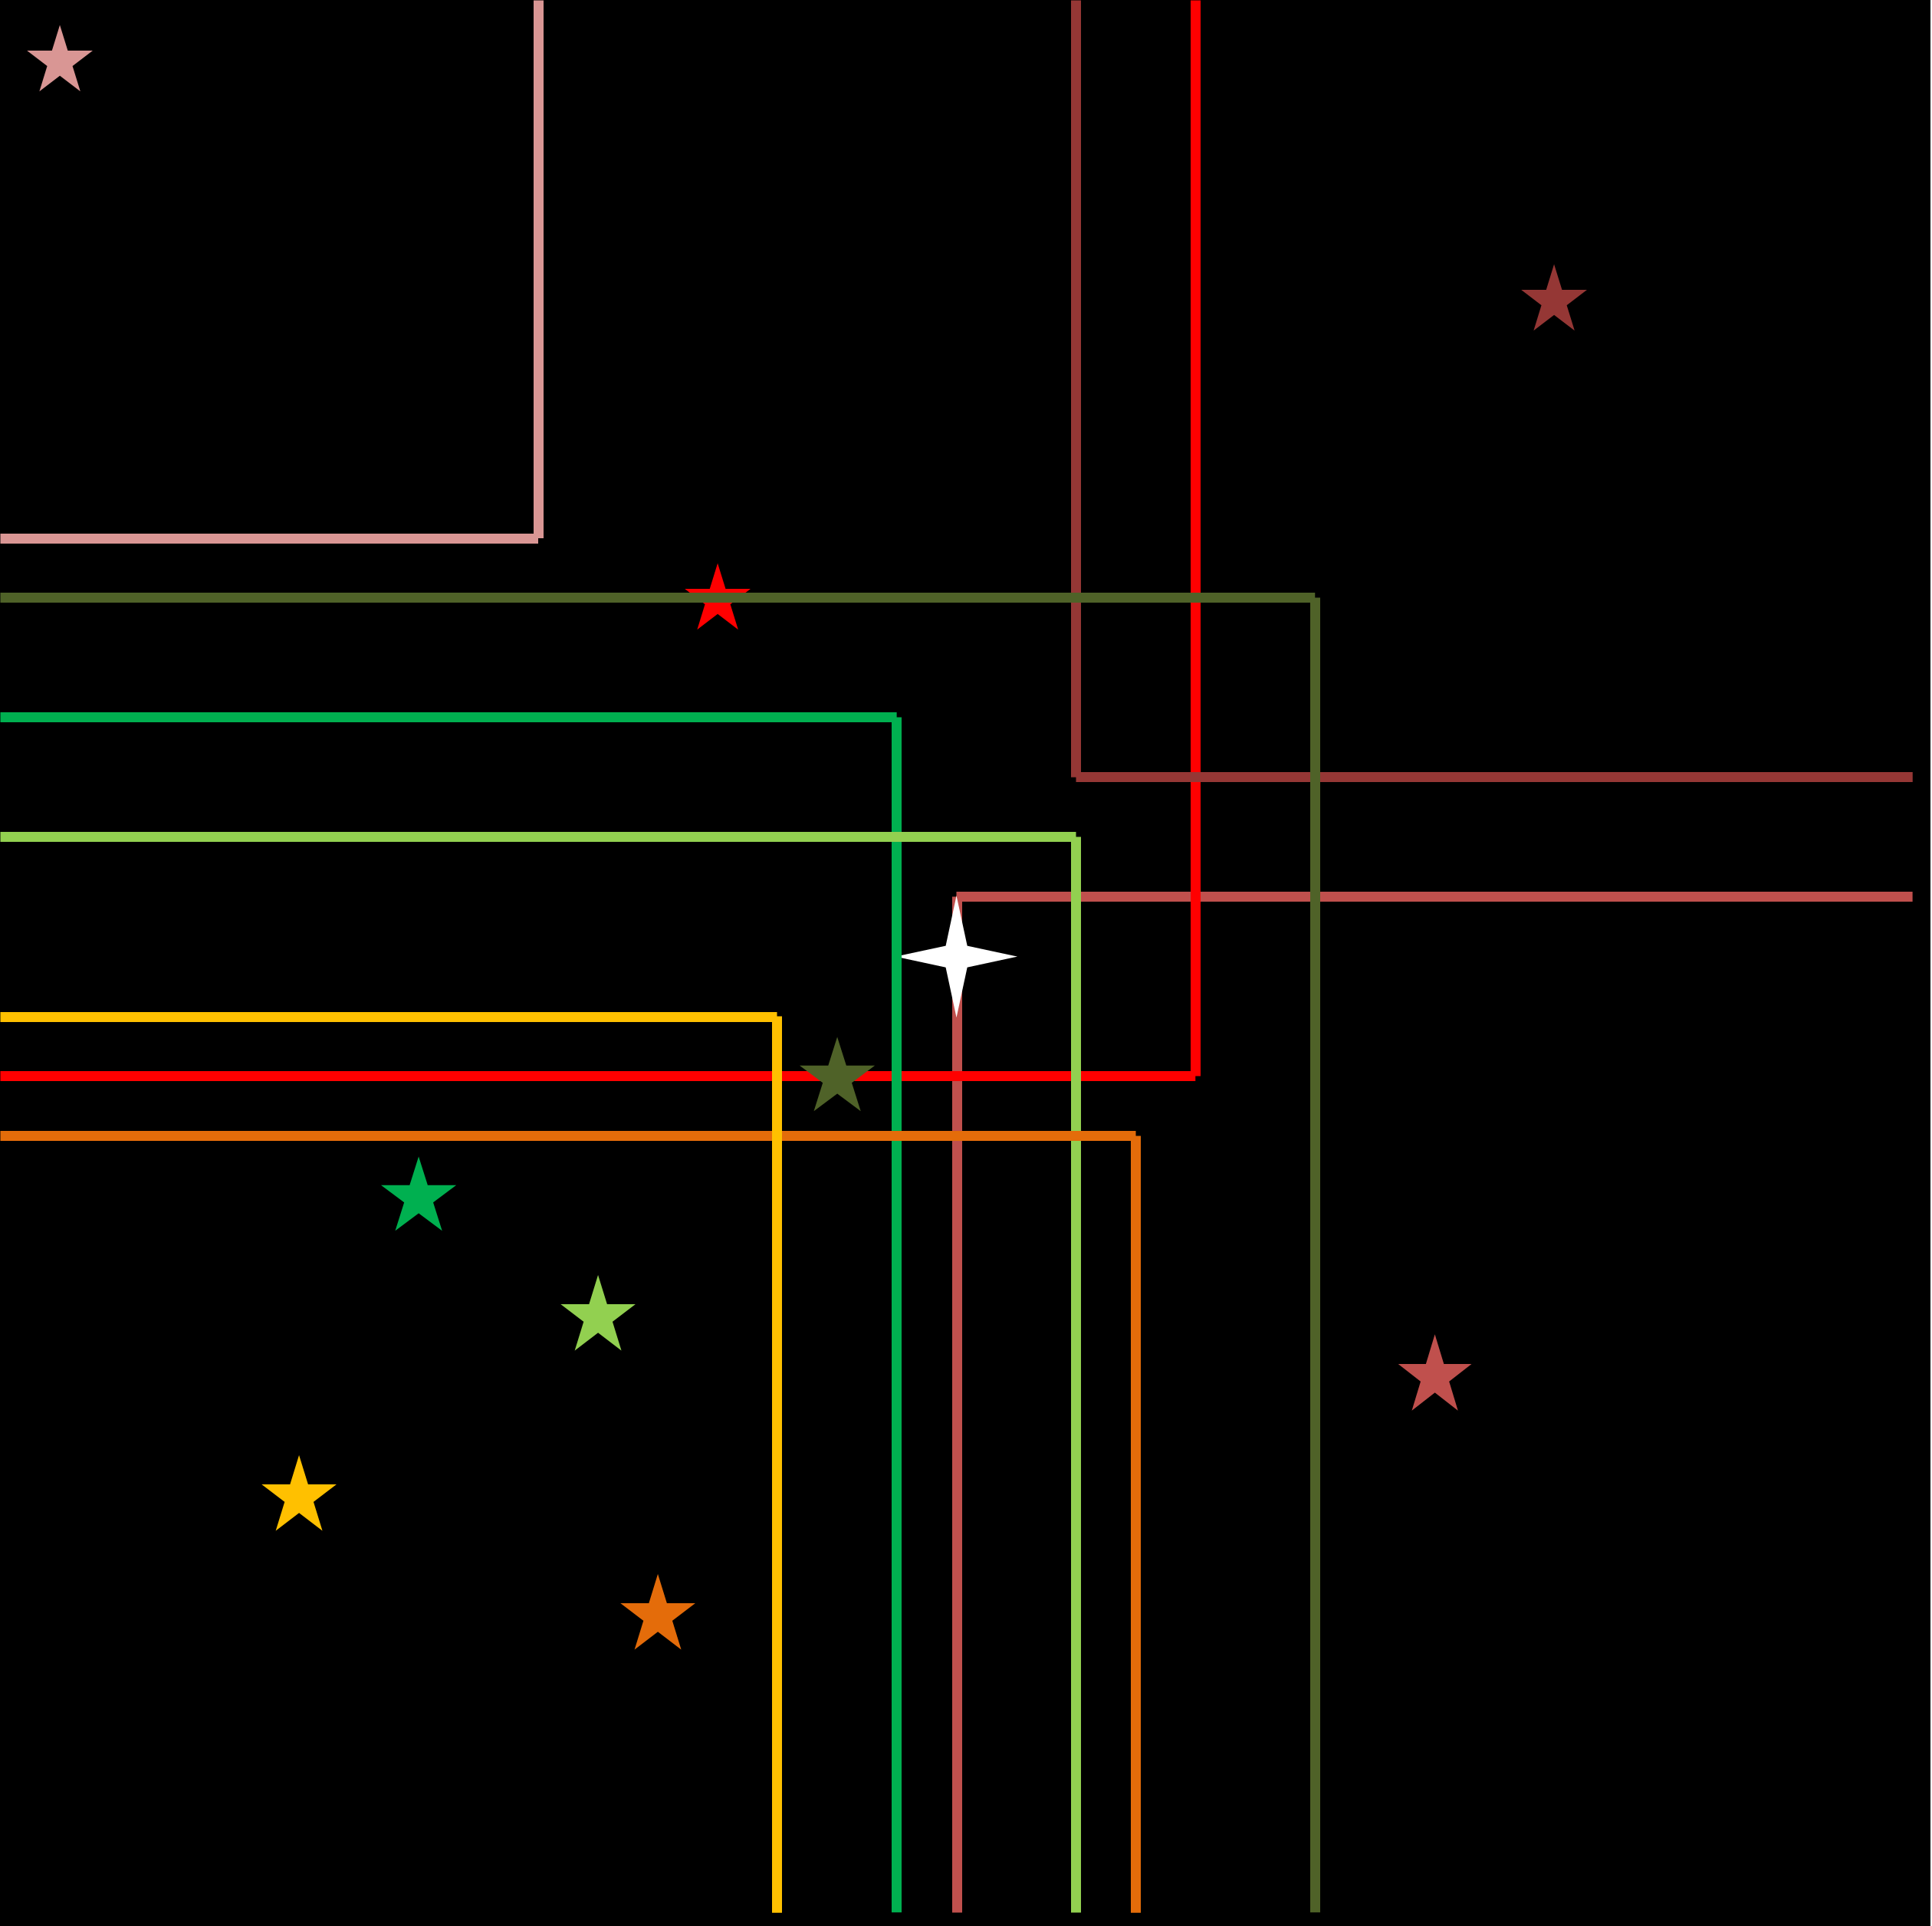
\includegraphics{fig3.png}}
\caption{\label{effective_locus}Each effective locus is defined by assigning a pair
of RA and Dec coordinates for a corner point and a pair of lines North
or South and East or West from the corner point. In this diagram, each
candidate reference star is assigned a colour, and the effective locus
that corresponds to it is drawn in the same colour. Copied from \citet{creaner2016thesis}}
\end{figure}

Specifically, the effective locus can be defined as a corner point of
the locus and two lines: one of constant RA and the other of constant
Dec emanating from the corner point. 

Using the Equatorial Coordinate System discussed in Section \ref{definition-of-coordinate-system-and-locus}, with
coordinates of the target specified by \((RA_t, Dec_t)\)
and coordinates of the candidate reference star defined by
\((RA_r, Dec_r)\) and a size of FoV of horizontal
length R and vertical length S, the coordinates of the corner point
\((RA_c, Dec_c)\) are defined as shown in Expression \ref{CPDef}.
\begin{equ}[!h]
  \begin{equation}
\begin{split}
&RA_t \leq RA_r \Rightarrow RA_c = RA_r- {\frac{R^\prime}{2}}\\
&RA_t > RA_r \Rightarrow RA_c = RA_r+ {\frac{R^\prime}{2}} \\
&Dec_t \leq Dec_r \Rightarrow Dec_c = Dec_r- {\frac{S}{2}}\\
&Dec_t > Dec_r \Rightarrow Dec_c = Dec_r + {\frac{S}{2}}
\end{split}
  \end{equation}
\caption{\label{CPDef}Definition of the corner point (\(RA_c\), \(Dec_c\)) of the effective locus for a FoV of size R x S for a candidate reference star at (\(RA_r\), \(Dec_r\)) and a target at (\(RA_t\), \(Dec_t\)) }
\end{equ}
The directions \(DirRA\) (the direction of the line of constant RA) and 
\(DirDec\) (the direction of the line of constant Dec) of the lines is
determined by the RA and Dec of the candidate
reference star relative to that of the target are given in Expression \ref{DirDef} and as described below.

\begin{itemize}
\tightlist
\item
  If the RA of the candidate is greater than the target, the line of
  constant Dec is drawn in the direction of increasing RA
\item
  If the RA of the candidate is less than the target, the line of
  constant Dec is drawn in the direction of decreasing RA
\item
  If the Dec of the candidate is greater than the target, the line of
  constant RA is drawn in the direction of increasing Dec
\item
  If the Dec of the candidate is less than the target, the line of
  constant RA is drawn in the direction of decreasing Dec.
\end{itemize}

\begin{equ}[!h]
  \begin{equation}
\begin{split}
&RA_t \leq RA_r \Rightarrow DirDec = +ive\\
&RA_t > RA_r \Rightarrow DirDec = -ive \\
&Dec_t \leq Dec_r \Rightarrow DirRA = +ive\\
&Dec_t > Dec_r \Rightarrow DirRA =-ive
\end{split}
  \end{equation}
\caption{\label{DirDef}Definition the directions (\(DirRA\), \(DirDec\)) of the lines from the corner point of that define the effective locus for a FoV of size R x S for a candidate reference star at (\(RA_c\), \(Dec_c\)) and given a target at (\(RA_t\), \(Dec_t\)).  In current implementations, these values are encoded as a binary switch, with 1 representing increasing (\(+ive\)) direction and 0 representing decreasing (\(-ive\)) direction.}
\end{equ}



\hypertarget{identifying-and-scoring-points-of-intersection-and-identifying-the-pointing.}{%
\subsection{Identifying and Scoring Points of Intersection and
identifying the
pointing.}\label{identifying-and-scoring-points-of-intersection-and-identifying-the-pointing.}}

The points where lines from any two loci are identified. This involves
comparing the corner point RA and Dec and direction of lines for one
locus with the corner point RA and Dec and direction of lines for a
second locus. In total eight variable associated with each two loci are
checked:

\begin{itemize}
\tightlist
\item
  For Locus 1: \(RA_{c1}\), \(Dec_{c1}\), \(DirRA_1\), \(DirDec_1\)
\item
  For Locus 2: \(RA_{c2}\), \(Dec_{c2}\), \(DirRA_2\), \(DirDec_2\)
\end{itemize}

Using these parameters, a check as to whether an intersection between
the two loci occurs is achieved as follows:

\begin{itemize}
\tightlist
\item
  A line of constant Dec in the positive RA direction from the corner
  point of locus 1 will intersect with a line of constant RA in the
  positive Dec direction from the corner point of locus 2 if locus 1 has
  a lower RA than locus 2 and locus 1 has a higher Dec than locus 2.
\item
  A line of constant RA in the positive Dec direction from the corner
  point of locus 1 will intersect with a line of constant Dec in the
  positive RA direction from the corner point of locus 2 if locus 1 has
  a lower Dec than locus 2 and locus 1 has a higher RA than locus 2.
\end{itemize}

\ldots{} and so on. By checking all such possible combinations, all
pairs of loci in the field which result in a Point of Intersection are
identified and their RA and Dec noted.

\begin{figure}[!htb]
\centering
\colorbox{black}{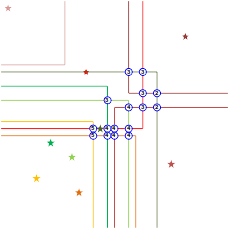
\includegraphics{fig4.png}}
\caption{\label{PoIscores}Points of Intersection (PoI), and their associated
score. In this diagram each star has a rating of 1, hence the score
associated with each PoI is equal to the number of reference stars
within a FoV centred at that PoI.Copied from \citet{creaner2016thesis}}
\end{figure}
Subsequent to identification, each Point of Intersection is then scored.
This is achieved as follows:

\begin{itemize}
\tightlist
\item
  The number of reference stars in the Field of View centred on the
  Point of Intersection is counted.
\item
  Each reference star is assigned a \(rating\) value between 0 and 1 based
  on its similarity in colour to the target.
\item
  The ratings from all counted reference stars in the Field of View are
  combined into one overall score for the field (Figure \ref{PoIscores}).
\item
  The Point of Intersection with the highest score becomes the pointing
  for the target (Figure \ref{final}).
\end{itemize}


\begin{figure}[!htb]
\centering
\colorbox{black}{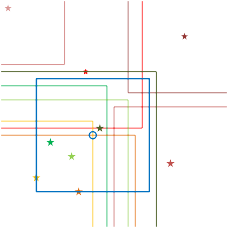
\includegraphics{fig5.png}}
\caption{\label{final}Locus Algorithm. Target: white star. Pointing \& FoV:
blue. Reference stars and their loci: Fully in the FoV: greens. On the
edge of the FoV: yellows. Outside FoV: reds.  Modified from \citet{creaner2016thesis}}
\end{figure}

Scenarios can arise which result in an inability to identify an optimum
pointing for a given target for example if there are no, or a maximum of
one reference stars in the candidate zone; and if no points of
intersection arise -- a scenario which can arise if two (or more)
reference fall in one quadrant of the candidate zone resulting in
concentric loci, or where reference stars are too far apart in different
quadrants of the candidate zone in order for their loci to intersect.
All four of these scenarios are considered in practical implementations
of the locus algorithm aimed at identifying the optimum pointings for a
set of targets in a catalogue or list of targets.

In summary, the Locus Algorithm successfully identifies the RA and Dec
coordinates of the optimum pointing for a given target, where optimum
means a field of view with the maximum number of reference stars which
are similar in magnitude and colour to the target.

\newpage

\hypertarget{example-implementation-of-the-locus-algorithm}{%
\section{Example Implementation of the Locus
Algorithm}\label{example-implementation-of-the-locus-algorithm}}

To illustrate the workings of the Locus Algorithm, a worked example is
given here. The star with SDSS ID 1237680117417115655 (RA = 346.65 and
DEC = -5.04) is used as the example. This star has SDSS magnitudes as
given in the table below.

\begin{longtable}[]{@{}lr@{}}
\toprule
Band & SDSS\_Magnitude\tabularnewline
\midrule
\endhead
u & 17.20\tabularnewline
g & 15.38\tabularnewline
r & 14.65\tabularnewline
i & 14.40\tabularnewline
z & 14.28\tabularnewline
\bottomrule
\end{longtable}

The telescope system considered has parameters given in the table below:

\begin{longtable}[]{@{}lr@{}}
\toprule
Parameters & Values\tabularnewline
\midrule
\endhead
Field of View in minutes & 10.00\tabularnewline
Resolution Limit in minutes & 0.18\tabularnewline
Dynamic Range in magnitudes & 2.00\tabularnewline
\bottomrule
\end{longtable}

The potential reference stars are selected as follows:

\begin{itemize}
\tightlist
\item
  Position: Within the Candidate Zone, SDSS records 1345 separate
  objects.
\item
  Magnitude: the reference star must be within the dynamic range, 2, of
  the target's magnitude of 14.648. This leaves 41 potential references.
\item
  Colour: the reference star must match the colour of the target to
  within a user-specified limit. In this case this means \(g - r\)
  between 0.634 and 0.834 and \(r - i\) between 0.149 and 0.349 This
  leaves 15 potential references.
\item
  Resolvability: the reference star must be resolvable, i.e.~no other
  star that would impact a brightness measurements within a
  user-specified resolution limit, in this case 11 arc seconds. Any
  object this close to a potential reference star and with an r-band
  magnitude which is 5 magnitudes greater than the potential reference
  or brighter will pollute the light from the potential reference star.
  This leaves 14 potential references.
\end{itemize}

After checking different fields of view, a pointing with RA = 346.65 and
DEC = -5.12 included both the target and 7 reference stars. These
numbers are presented in the table below.

\begin{longtable}[]{@{}lr@{}}
\toprule
filters & numbers\tabularnewline
\midrule
\endhead
Position, in Field of View & 1345\tabularnewline
Correct Magnitude & 41\tabularnewline
Correct Colour & 15\tabularnewline
Resolvable & 14\tabularnewline
In Final Field of View & 7\tabularnewline
\bottomrule
\end{longtable}

\newpage

The SQL query to download potential reference stars from SDSS is given
below. This SQL query is run on the CAS database, release DR15, of SDSS.
Note the flags to give clean photometry (Aguado et al. (2018))

SELECT objID, ra, dec, psfmag\_u, psfmag\_g, psfmag\_r, psfmag\_i,
psfmag\_z\\
FROM photoObj\\
WHERE (ra between ( 346.48270496969 ) AND ( 346.817331746246 )\\
OR ra BETWEEN ( 706.48270496969 ) AND ( 706.817331746246 )\\
OR ra BETWEEN ( -13.5172950303096 ) AND ( -13.1826682537544 ))\\
AND dec BETWEEN ( -5.20597532982638 ) AND ( -4.87264199649304 )\\
AND psfmag\_r BETWEEN 12.64849 AND 16.64849\\
AND (psfmag\_g - psfmag\_r) BETWEEN ( 0.633989999999999 ) AND (
0.833989999999999 )\\
AND (psfmag\_r - psfmag\_i) BETWEEN ( 0.149080000000001 ) AND (
0.349080000000001 )\\
AND clean = 1\\
AND (calibStatus\_r \& 1) != 0

A table with the reference stars in the final field of view is given
below:

\begin{longtable}[]{@{}lrrrrrrrr@{}}
\toprule
objID & ra & dec & mag\_u & mag\_g & mag\_r & mag\_i & mag\_z &
ratings\tabularnewline
\midrule
\endhead
1237680117417050120 & 346.563 & -5.153 & 18.460 & 16.498 & 15.771 &
15.533 & 15.397 & 0.830\tabularnewline
1237680117417050133 & 346.594 & -5.161 & 16.702 & 14.825 & 14.068 &
13.887 & 13.648 & 0.241\tabularnewline
1237680117417115655 & 346.650 & -5.039 & 17.199 & 15.382 & 14.648 &
14.399 & 14.281 & 1.000\tabularnewline
1237680117417115762 & 346.676 & -5.120 & 18.920 & 17.022 & 16.282 &
15.974 & 15.851 & 0.380\tabularnewline
1237680065348435996 & 346.707 & -5.199 & 16.704 & 14.699 & 13.905 &
13.676 & 13.515 & 0.322\tabularnewline
1237680117417115683 & 346.713 & -5.050 & 17.585 & 15.782 & 15.109 &
14.867 & 14.798 & 0.361\tabularnewline
1237680117417115692 & 346.724 & -5.047 & 18.362 & 16.576 & 15.843 &
15.568 & 15.464 & 0.734\tabularnewline
\bottomrule
\end{longtable}

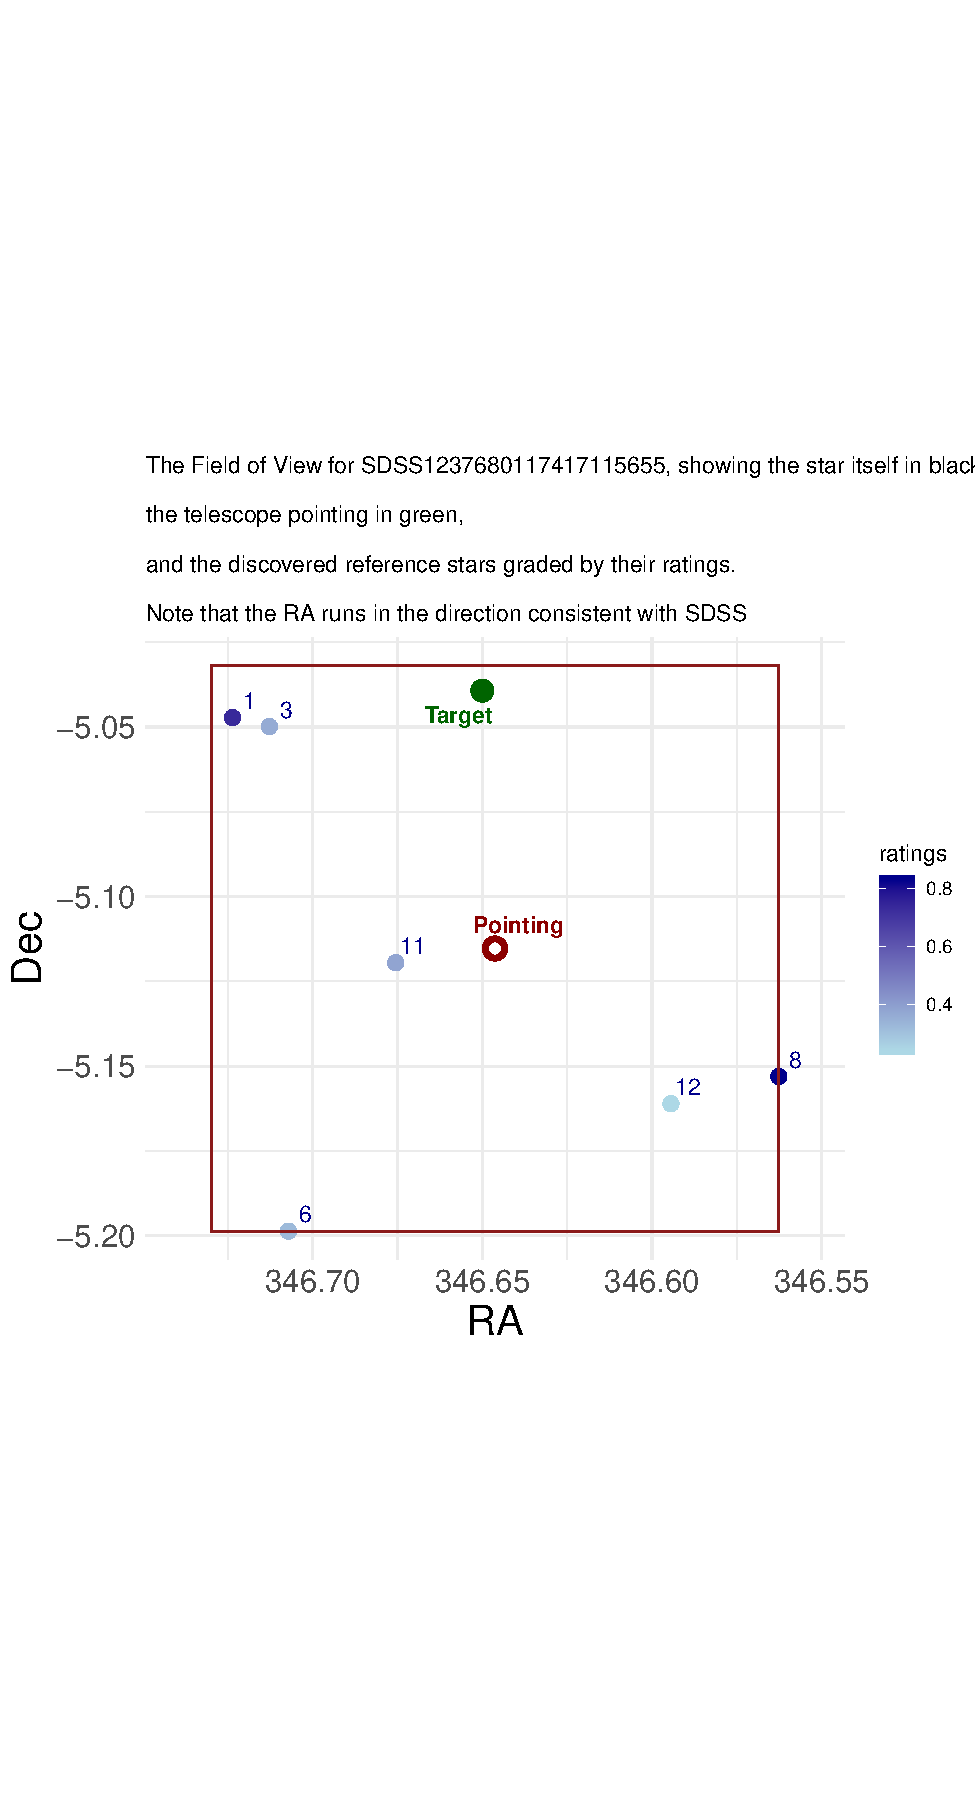
\includegraphics{Locus_Whole_files/figure-latex/locus_plot-1.pdf}

%% References with BibTeX database:

\bibliographystyle{elsarticle-num-names}
\bibliography{Locus_Whole_bibtex}


%\newpage
%
%\hypertarget{references}{%
%\subsection*{References}\label{references}}
%\addcontentsline{toc}{subsection}{References}
%
%\hypertarget{refs}{}
%\leavevmode\hypertarget{ref-Aguado2018}{}%
%Aguado, D. S., Romina Ahumada, Andres Almeida, Scott F. Anderson, Brett
%H. Andrews, Borja Anguiano, Erik Aquino Ortiz, et al. 2018. ``The
%Fifteenth Data Release of the Sloan Digital Sky Surveys: First Release
%of MaNGA Derived Quantities, Data Visualization Tools and Stellar
%Library,'' December. \url{https://doi.org/10.3847/1538-4365/aaf651}.
%
%\leavevmode\hypertarget{ref-Honeycutt1992}{}%
%Honeycutt, R. K. 1992. ``CCD ensemble photometry on an inhomogeneous set
%of exposures.'' \emph{Publications of the Astronomical Society of the
%Pacific} 104 (676). IOP Publishing: 435.
%\url{https://doi.org/10.1086/133015}.
%
%\leavevmode\hypertarget{ref-Howell2000}{}%
%Howell, Steve B., and Steve B. 2000. ``Handbook of CCD Astronomy.''
%\emph{Handbook of CCD Astronomy / Steve B. Howell. Cambridge, U.K. ; New
%York : Cambridge University Press, C2000. (Cambridge Observing Handbooks
%for Research Astronomers ; 2)}.
%\url{http://adsabs.harvard.edu/abs/2000hccd.book.....H}.
%
%\leavevmode\hypertarget{ref-Milone2011}{}%
%Milone, E. F., and Jan Willem Pel. 2011. ``The High Road to Astronomical
%Photometric Precision: Differential Photometry.'' In \emph{Astronomical
%Photometry: Past, Present, and Future, Edited by E.f. Milone and c.
%Sterken. Astrophysics and Space Science Library, Vol. 373. Berlin:
%Springer, 2011. ISBN 978-1-4419-8049-6, P. 33-68}, 373:33--68.
%\url{https://doi.org/10.1007/978-1-4419-8050-2_2}.
%
%\leavevmode\hypertarget{ref-YOUNG1991}{}%
%YOUNG, ANDREW T., RUSSELL M. GENET, LOUIS J. BOYD, WILLIAM J. BORUCKI,
%G. WESLEY LOCKWOOD, GREGORY W. HENRY, DOUGLAS S. HALL, et al. 1991.
%``PRECISE AUTOMATIC DIFFERENTIAL STELLAR PHOTOMETRY.'' Astronomical
%Society of the Pacific. \url{https://doi.org/10.2307/40679676}.

\end{document}


